% !TEX root = main.tex

\section{Développement de méthodes permettant l'adaptation du filtre de Kalman d'ensemble avec des simulations sans maillage}

\subsection{Objectif}
Le filtre de Kalman présenté en Section~\ref*{sec:enkf} est un filtre séquentiel adéquat pour appliquer des méthodes d'assimilation pour des modèles de grande dimension et non-linéaire. Il consiste à mettre à jour un ensemble d'état en déterminant un gain de Kalman pour combiner l'état prédit et un terme d'innovation fonction de l'erreur de prédiction. En particulier ce gain va dépendre des statistiques du champ.

\subsection{Mise à jour défini dans l'espace d'observation}

La mise à jour du filtre de Kalman se base sur l'approximation des statistiques des distributions de l'état et des observations pour approché le gain de Kalman (voir \eqref{eq:enkf_formula}).

Dans le cas d'un état qui repose sur une discrétisation particulaire, on ne peut directement évaluer ses statistiques directement sur les quantités particulaires, c'est à dire positions et intensité. En effet, chaque membre possède


Heureusement La particularité du filtre de Kalman d'ensemble est qu'il fait une approximation de faible rang du gain de Kalman. Nous avons montré en Section~\ref{sec:faible_rang} que la mise à jour s'exprimait comme une combinaison des états de l'ensemble $X$.

De cette manière la mise à jour est déterminé comme

\begin{equation*}
    \mstate_a = \mstate_f + \mstate_f \Fcorr, \quad \Fcorr = \frac{1}{\sqrt{N-1}} \annomY_f^T {(\annomY_f \annomY_f^T + \bm R)}^{-1}(\mdata - \mpred).
\end{equation*}.

Où la matrice de correction $\Fcorr \in $ est indépendante de la discrétisation.

Cette indépendance est possible par la linéarisation de l'opérateur d'observation et l'approche par rang faible. D'autres versions du filtre EnKF offre les mêmes propriétés. C'est le cas du \textit{ensemble transform Kalman filter} (ETKF, \cite{Hunt2007}). En effet, ce filtres travaillent directement dans l'espace de perturbation.

Travailler dans l'espace de perturbation des observations $\bm Y^T$ permet d'éviter d'exprimer les statistiques de l'état.

L'étape d'analyse est donc une combinaison qui ne dépend que des observations $\bm y$ (perturbé pour le filtre stochastique), les prédictions de l'ensemble $\left[\mathcal{H}(x^i_f)\right]_{i=1}^{N}$, et la matrice de covariance d'erreur $R^{1}$. De cette manière, pour chaque membre $i$, le champ analysé $\fstate_i^a$ peut être déterminé en tout point de l'espace $\bm x \in \omega$ grâce aux champs prédits $\fstate_j^f$ tel que

\begin{equation*}
    \fstate_i^a(\bx) =\fstate_i^f(\bx) + \sum_{j=1}^{N} F_{ji} \fstate_j ^f(\bx), \quad i = 1, \dots, N.
\end{equation*}

\subsection{Mise à jour comme solution particulaire}

Les solutions analysées peuvent être décomposées à partir de la discrétisation particulaire des champs $\fstate_i^f$.

Dans un premier temps, nous supposons que les positions de particules sont les mêmes pour tous les membres. On note $(\bx_1,...\bx_{N_p}) \in \mathbb{R}^d$ les positions des centres de particule, deux à deux distincts de telle sorte que, pour tout $\bx \in \mathbb{R}^d$

\begin{eqnarray*}~\label{eq:enkf_formula_same_part}
    \fstate_i^a(\bx) &=& \fstate_i^f(\bx) + \sum_{j=1}^{N} F_{ji} \fstate_j ^f(\bx) \\
    &=& \sum_{p=1}^{N_p} \Gamma^f_{p,i} \phi_{\varepsilon}(\bx - \bx_p) + \sum_{j=1}^{N} F_{ji} \sum_{p=1}^{N_p} \Gamma_j ^f(\bx) \phi_{\varepsilon}(\bx - \bx_p) \\
    &=& \sum_{p=1}^{N_p} \left[\Gamma^f_{p,i} + \sum_{j=1}^{N} F_{ji} \Gamma^f_{p,j} \right] \phi_{\varepsilon}(\bx - \bx_p).
\end{eqnarray*}

En utilisant la linéarité de la décomposition par rapport aux intensités $\Gamma^f_{p}$, l'analyse pour chaque membre peut directement s'exprimer pour chaque membre en appliquant la mise à jour directement sur les intensités. En notant $\bm \Gamma$ la matrice dont la i-ème colonne est $(\Gamma_{1, i},...\Gamma_{N_p, i})$, la mise à jour est directement exprimé comme

\begin{equation*}
    \bm \Gamma^a = \bm \Gamma + \bm \Gamma \bm F.
\end{equation*}

Cependant, dans le cas général les positions de particules diffèrent d'un membre à l'autre. Dans ce cas, en utilisant la décomposition particulaire des champs prédit $\mP_i^f$, la solution analysée va s'exprime comme

\begin{eqnarray*}
    \fstate_i^a(\bx) &=& \sum_{p \in \mP_i^f}\Gamma^f_p \phi_{\varepsilon}(\bx - \bx_p) + \sum_{j=1}^{N} F_{ji}  \sum_{p' \in \mP_j^f}\Gamma^f_{p'} \phi_{\varepsilon}(\bx - \bx_{p'}) \\
    &=& \sum_{p \in \mP_i^f}\left[(1 + F_{ii})\Gamma^f_p \phi_{\varepsilon}(\bx - \bx_{p})\right]   + \sum_{j\neq i} F_{ji} \Gamma^f_{p'} \phi_{\varepsilon}(\bx - \bx_{p'})\\
    &=& \sum_{p \in \mP_i^f} \Gamma^a_p \phi_{\varepsilon}(\bx - \bx_p).
\end{eqnarray*}
$\fstate_i^a$ est bien une solution particulaire.


Sans perte de généralité, en supposant que chaque particules ont des positions $x_p$ distincts, alors l'espace d'approximation est de dimension $\sum_{i=1}^{N} \text{Card}(\mathcal{P}^f_i)$.

Ainsi, à chaque étape d'assimilation de données, le nombre de particule pour approcher la solution analysée augmente exponentiellement avec l'union des particules de tous les membres comme en Figure~\ref{fig:support_particles}.

\begin{figure}~\label{fig:support_particles}
    \centering
    \begin{subfigure}{0.5\textwidth}
        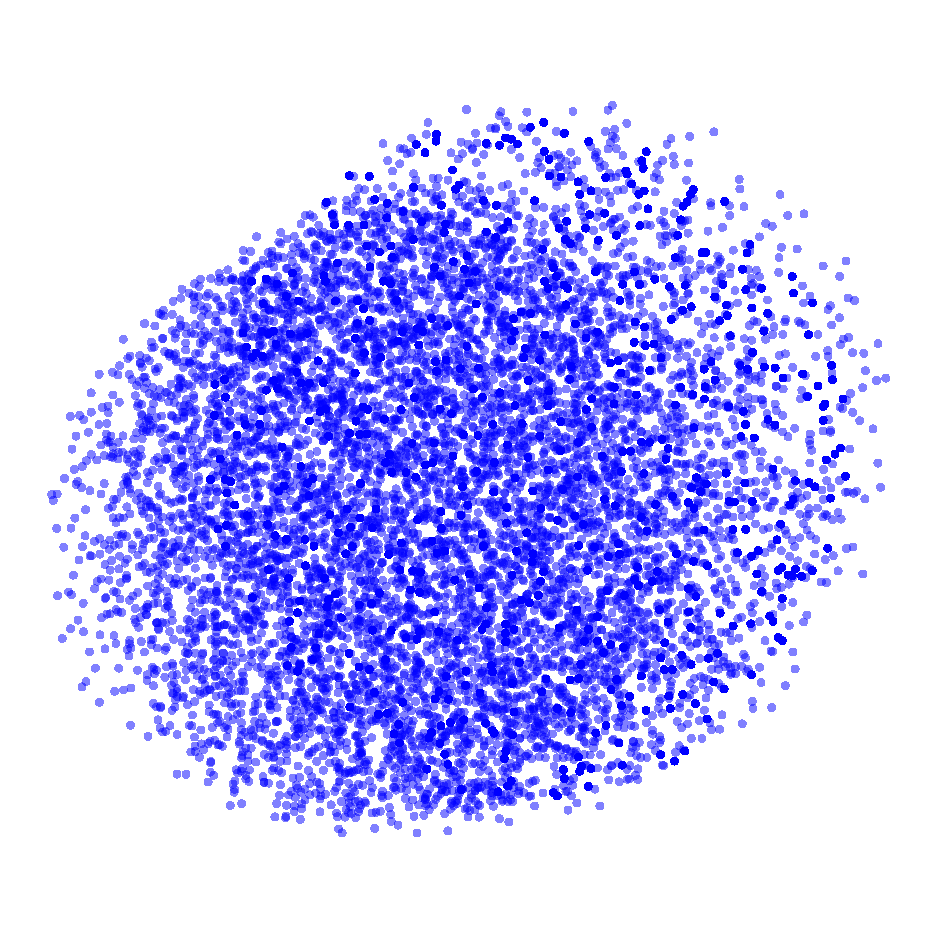
\includegraphics[width=\textwidth]{./images/all_particles.pdf}
    \end{subfigure}
    \begin{subfigure}{0.5\textwidth}
        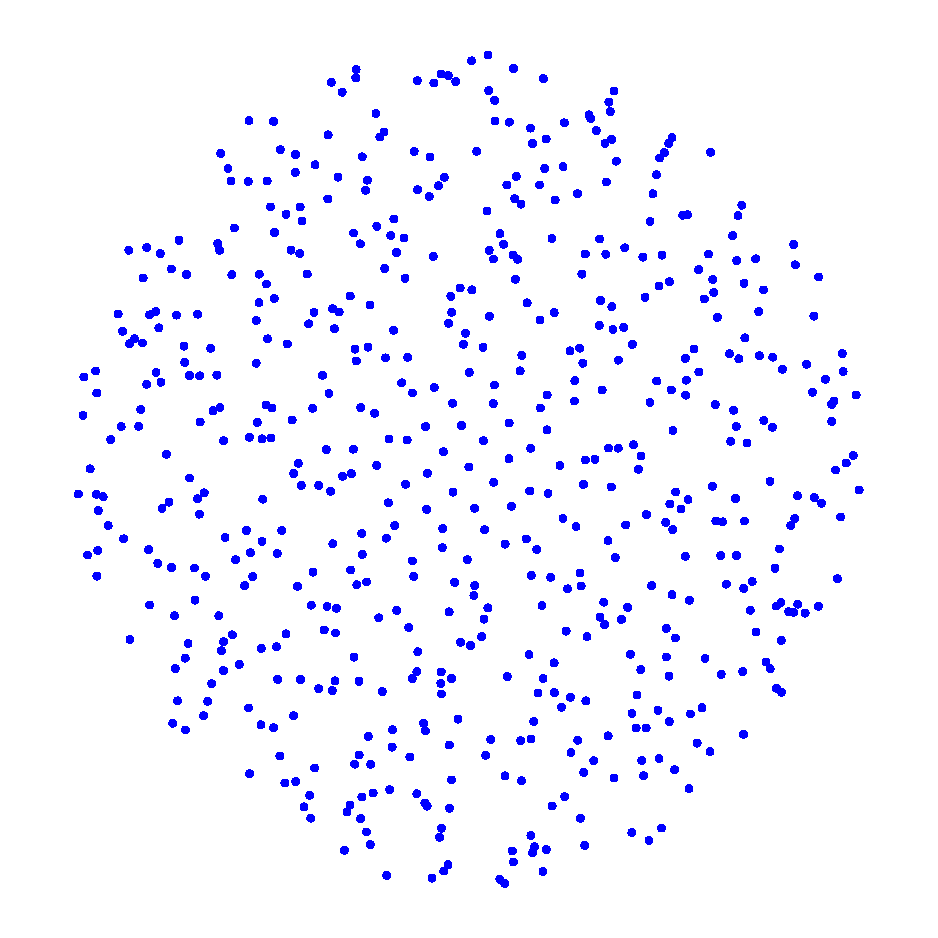
\includegraphics[width=0.5\textwidth]{./images/memb_particles.pdf}
    \end{subfigure}
    \caption{Support de particule d'un membre avant et après correction.}
\end{figure}

Cette mise à jour ne peut donc pas être mise en pratique. Il est nécessaire de proposer des méthodes pour réduire le nombre de particules pour représenter la solution analyser. Afin de résoudre ce problème, nous proposons deux approches distinctes:

\begin{itemize}
    \item \textbf{Remesh-EnKF}: \\
    \item \textbf{Part-EnKF}: \\
\end{itemize}

\subsection{Remesh-EnKF : Générer une même configuration particulaire}

Cette méthode consiste à revenir à un ensemble de particules définis sur un support commun. En remaillant régulièrement, nous pouvons contrôler et limiter le nombre de particules, assurant ainsi une représentation plus homogène et gérable de la solution. Le remaillage permet de maintenir une distribution équilibrée des particules, tout en préservant les caractéristiques essentielles de la solution originale.

\subsubsection*{Méthode de remaillage pour obtenir un support de particule commun}

La méthode de remaillage est une technique essentielle dans notre approche pour maintenir un support de particule uniforme parmi tous les membres de la solution. À l'origine développée pour atténuer les distorsions dans la distribution des particules, cette méthode se fonde sur un schéma de redistribution sur une grille régulière de particules, utilisant des opérateurs de projection et d'interpolation. Ce processus permet de passer d'une représentation lagrangienne à une représentation eulérienne, puis ensuite revenir à une représentation lagrangienne.

L'essence de cette méthode réside dans l'utilisation d'opérateurs similaires à ceux employés par les méthodes Particles in Cell (PIC) comme la méthode \textit{Vortex-In-Cell} (VIC) ou la \textit{Material Point Method} (MPM).

Le remaillage est défini en deux étapes.

Consiste en un schéma de redistribution sur une grille régulière de particules à l'aide d'opérateur de projection et d'interpolation. Elle consiste à passer d'une représentation lagragienne à eulérienne, puis de revenir sur une grille de particules lagrangienne. En fait même type d'opérateur qu'utilisé par les méthodes particules in cell (PIC).

Dans notre méthodologie, nous proposons une approche en deux étapes. Tout d'abord, nous effectuons une étape d'assignation (\ref{assigment}) pour transférer la discrétisation des particules à une discrétisation sur une grille. Ensuite, une étape d'interpolation (\ref{interpolation}) est réalisée pour obtenir un nouvel ensemble de particules régulièrement espacées.

Notre analyse se rapporte au scénario unidimensionnel, où $\Omega \in \mathbb{R}$. L'extension au cas $n$-dimensionnel peut être réalisée par la tensorisation de l'approche unidimensionnelle.

\begin{enumerate}[label=(\alph*)]
    \item \textit{Affectation sur une grille eulérienne} \label{assigment}

          Nous désignons par $z_{I}$ et $z_{p}$ respectivement les emplacements sur la grille et les anciens emplacements des particules. Les nouvelles particules sont définies sur une grille de $n_g$ éléments avec un espacement régulier $\ell_I = 2 d_p$, où $d_p$ est la taille caractéristique des particules. Nous définissons les intensités des particules comme $\bm U_p$ et les valeurs du champ nodal comme $\bm u_I$. En utilisant une fonction de forme $W$, l'étape d'affectation des particules à chaque nœud $I \in \Lambda$ peut être écrite comme

          \[
              \bm{u}_I = \frac{1}{V_I} \sum_{p \in \mathcal{P}} \bm U_p  W \left(\frac{z_I - z_p}{\ell_I} \right).
          \]

          Où $W$ détermine une redistribution de l'intensité sur la grille, la nouvelle discrétisation peut ensuite être utilisée pour approximer le champ $\bm{u}_p$, défini par la discrétisation des particules par interpolation

          \[
              \bm{u}_p(z) \approx \bm{u}_g(z) = \sum_{I \in \Lambda} \bm u_I W \left(\frac{z - z_I}{\ell_I} \right) \quad \forall z \in \Omega.
          \]

    \item \textit{Interpolation sur une nouvelle discrétisation régulière des particules} \label{interpolation}

          Un nouvel ensemble de particules est défini au quart de chaque cellule de sorte que la nouvelle position est définie à $z_{p'} = d_p/2 + i~dp, \quad i = 0,\dots, 2n_g $. La valeur du champ est alors interpolée à cette nouvelle position et multipliée par le volume de la particule $\bm{U}_{p'} = \bm  u_g(z_{p'}) V_{p'}$ afin de donner une nouvelle approximation particulaire de ce champ

          \[
              \bm{u}_g(z)  \approx \bm{u}_{p'}(z) = \sum_{p'\in\mathcal{P'}} \bm{u}_g(z_{p'}) V_p,
          \]

\end{enumerate}

La combinaison de ces deux étapes peut être initialement utilisée pour générer une nouvelle distribution de particules non déformées. La fonction de forme $W$ détermine le type et la qualité du transfert. Le critère de la qualité de la méthode réside dans la conservation des premiers moments des distributions de particules, comme détaillé en Annexe~\ref{appendix:momentConservation}.

Pour $W$, on peut utiliser une fonction d'interpolation afine, qui garantit la conservation du moment 0. Pour une conservation des moments supérieurs, la fonction B-spline fournit une fonction de lissage d'ordre plus élevé.

Monaghan~\cite{monaghan_extrapolating_1985} propose une approche systématique pour améliorer la précision et maintenir la régularité par extrapolation. Le concept implique la construction d'une nouvelle fonction de forme basée sur une coupure et sa dérivée radiale. Pour $m = 4$, la B-spline cubique est améliorée par le noyau d'interpolation suivant

\begin{eqnarray*}~\label{cubic_radial_kernel}
    M_4'(z) &=& \left{ \begin{aligned}
         & 1 - \frac{5}{2}z^2 + \frac{3}{2} |z|^3 & 0 \leq & |z| \leq 1 & \
         & \frac{1}{2}{(2 - |z|)}^2(1 - |z|)      & 1 \leq & |z| \leq 2 & \
         & 0                                      & 2 \leq & |z|.
    \end{aligned}
    \right.
\end{eqnarray*}

que nous utiliserons dans les applications.

Enfin, dans l'espace multidimensionnel, le noyau de redistribution $W$ peut être obtenu comme le produit du noyau unidimensionnel appliqué à chaque coordonnée, comme suit

\begin{eqnarray*}
    \bm U_p &=& \sum_{I \in \Lambda} \bm U_I W \left(\bm z_p - \bm z_I, \ell_I \right) \
    &=& \sum_{I \in \Lambda} \bm U_I \prod_{i = 1}^d W_{1\text{D}} \left(\frac{\bm z_{I, i} - \bm z_{p, i}}{\ell_I} \right)
\end{eqnarray*}

Le schéma est illustré dans la Figure~\ref{fig:remaillage}

\begin{figure}~\label{fig:remaillage}
\end{figure}

\subsubsection*{Algorithme}

Le filtre Remesh-EnKF utilise les opérateurs précédemment définis pour appliquer la mise à jour de EnKF. L'assimilation est effectuée avec les étapes suivantes :

\begin{itemize}
\begin{itemize}
    \item \textit{propagation} : Les membres sont propagé, étant donné un nouvel ensemble de particules $\mathcal{P}^f_i = {(\bm z^f_{ip}, \bm U^f_{ip})}{ip = 1}^{N{ip}}$,
    \item \textit{projection}: Le champ associé est projeté sur une grille régulière de $n_g$ éléments de longueur caractéristique $\ell_{iI}= 2dp$. En utilisant l'opérateur de projection~\ref{assigment}, nous obtenons pour chaque noeud $iI \in \Lambda_{i}$
          \begin{equation*}
              \bm{u}^f_{iI} = \frac1{V_{iI}} \sum_{ip \in \mathcal P^f_i} \bm U^f_{ip} \bm W \left(\frac{\bm z_{iI} - \bm z^f_{ip}}{\ell_{iI}} \right)
          \end{equation*}
    \item \textit{analyse}: Sur la base de cette nouvelle discrétisation, la mise à jour EnKF est appliquée aux valeurs d'état nodal $\bm{u}^f_{iI}$, tel que l'état d'analyse $\bm{u}{iI}^a$ est
          \begin{equation*}
              \bm{u}^a{iI} = \bm{u}^f_{iI} + \sum_{j=1}^{N_{\text{ens}}} F_{ji} \bm{u}^f_{jI},
          \end{equation*}
    \item \textit{interpolation}: Une nouvelle discrétisation régulière des particules est initialisée. Deux particules par direction sont placées à l'intérieur de chaque cellule de la grille. Les nouvelles intensités de particules sont évaluées grâce à l'opérateur d'interpolation~\ref{interpolation}, tel que $ip' \in \mathcal P_i^a$
          \begin{equation*}
              \bm U_{ip'}^a = \sum_{iI \in \Lambda} \bm u^a_{iI} \left(\frac{\bm z_{iI} - \bm z_{ip'}}{\ell_{iI}} \right).
          \end{equation*}
\end{itemize}

Les différentes étapes sont résumés dans l'algorithm~\ref{algo:remesh_enkf}

\begin{algorithm}

    \caption{Remesh Filter analysis update}~\label{algo:remesh_enkf}

    \KwData{$\bm G \in \mathbb R^{n_g \times d}, \bm z^a \in \mathbb R^{2 n_g \times d}$ \tcp*[r]{grille}}
    \KwData{$\bm R \in\mathbb{R}^{m}$  \tcp*[r]{covariance des observations}}
    \KwIn{$\mathcal{P}^f_i= \{(\bm z^f_{ip}, \bm U^f_{ip})\}_{ip = 1}^{N_{ip}}, \quad i = 1, \dots, N_{\text{ens}}$ \tcp*[r]{forward discretizations}}
    \KwIn{ $\bm Y_f \in \mathbb{R}^{m \times N_{\text{ens}}}$ \tcp*[r]{the associate observation anomalies}}
    \KwIn{$\bm D \in \mathbb{R}^{m \times N_{\text{ens}}}$  \tcp*[r]{the perturbed observations}}

    $ \Fcorr = \annomY_f^T {(\annomY_f \annomY_f^T + \bm R)}^{-1}(\mdata - \mpred)$ \tcp*[r]{correction matrix}
    \SetKwFunction{proj}{Projection}
    \SetKwFunction{assign}{Assign}
    \ForEach{$i = 1, \dots, \nens $}{
        $\bm u[:,i] =$ \proj{$\mathcal{P}^f_i, \bm G$}
    }
    $\bm u = \bm u + \bm u \Fcorr$ \tcp*[r]{analysis update}
    \ForEach{$i = 1, \dots, \nens $}{
    $\bm z^a_{ip}, \bm U^a_{ip} = $ \assign{$\bm u[:,i]$}
    }
    \Return{$\mathcal{P}^a_i=\{\bm z^a_{ip}, U^a_{ip}\}_{ip = 1}^{N_{a}}, \quad i = 1, \dots, N_{\text{ens}}$ \tcp*[r]{analyse discretizations} }
\end{algorithm}


On remarque que tous les opérateurs que nous avons définis sont linéaire. Ainsi, effectuer la mise à jour sur la grille comme dans l'algorithme, ou bien sur les nouvelles particules comme dans l'équation~\eqref{eq:enkf_formula_same_part} est équivalent car la mise à jour lors de l'analyse, l'opération d'interpolation ainsi que la projection sont linéaires par rapport aux intensités.
Cependant, l'ordre de l'algorithme actuel permet de réaliser le minimum d'opération sur les espaces de lus faible dimension.


\subsection{Part-EnKF : Mise à des intensités}

% Dire que ici on souhaite pouvoir approcher la solution avec uniquement les particules du membre afin d'éviter l'accroissement excessif du nombre de particules. La méthode consiste à trouver les bonnes intensité. En agissant ainsi on souhaite présenter une méthode qui intervient directement sur les particules sans jamais changer leur configuration.

\subsection{Complexité}



----------------
D'autre part, dans la Section~\ref{sec:method_part}, nous avons montré la compatibilité des méthodes sans maillage pour l'assimilation de données séquentiel. Nous avons montré alors que les méthodes sans maillage discrétisant un milieu continu pouvait être mis à jour lors de l'assimilation en modifiant positions et intensités des particules.

Toutefois, la mise à jour du filtre de Kalman d'Ensemble est dépendante de la discrétisation de l'état de ses membres pour le calcul du gain de Kalman d'ensemble. De plus, la mise à jour du filtre de Kalman d'Ensemble est basé sur une combinaison linéaire des membres au travers du gain de Kalman d'ensemble, celle-ci entraîne une explosion du nombre de particules dans la définition de la solution analysée.

L'objectif de ce chapitre est donc de présenter un certain nombre d'adaptation du filtre de Kalman d'Ensemble qui puisse être appliquées à des simulations sans maillage.

Pour cela, nous reformulons tout d'abord l'expression de la mise à jour afin qu'elle soit indépendante de la définition de l'état.
Enfin, les solutions analysées étant des combinaisons linéaires des particules de l'ensemble des membres, nous proposons de développer des méthodes pour réduire l'augmentation exponentielle des particules.

\subsection{Formulation de la correction dans l'espace des membres}

\subsection{Filtre Remesh-EnKF}
\subsubsection{Méthode de remaillage}
\subsubsection{Définition du Filtre}
\subsection{Filtre Part-EnKF}
\subsubsection{Méthode de régression}
\subsubsection{Définition du Filtre}

\subsubsection{}

\subsection{Bilan}

Nous avons développé deux adaptations du filtre EnKF adaptées au cas des simulations particulaires. Celle-ci tienne compte d'une augmentation exponentielle de particules.
Ces deux adaptations Remesh-EnKF et Part-EnKF correspondent à deux paradigmes. Dans le premier cas, le choix a été fait de regénérer complètement la discrétisation à l'aide de méthode de transfert particule à grille et de remaillage. Dans le second cas, le choix a été fait de conserver la position des particules de chaque membre et d'approcher la solution analysée.
Si ces filtres offre des adaptations du filtre de Kalman d'Ensemble, ils semblent souffrir de plusieurs limitations inhérante à leur schéma. Dans la prochaine section, leur capacité d'assimilation va être vérifié sur plusieurs applications données.

\section{Evaluation de la capacité des méthodes développées à assimiler les données sur plusieurs applications}

Deux filtres dérivée de EnKF ont été développés. A l'aide deux deux applications basées sur une méthode


\subsection{Bilan}